The number of events observed in data in the signal regions was compared with
the background only fit. The results of the comparison between the observed
number of events in data and the background calculations including the
background only fit is shown in \cref{fig:sr_plots}. No significant excess of
data over background is observed. The results of the global fit procedure
described in Section~\ref{sec:glob-simult-likel} are used to set model
independent exclusion limit (see Section~\ref{sec:model-indep-limits}) and
interpreted in terms of squark pair production with
$\widetilde{q} \rightarrow q + \widetilde{\chi}_1^0\, (q = u,\, d,\, c,\, s)$
(see Section~\ref{sec:interpretation}).
\begin{figure}[!th]
  \centering
  \begin{subfigure}[t]{.48\linewidth}
    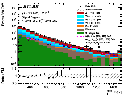
\includegraphics[width=\linewidth]{sr_et_miss}
    \caption{$\met$ distribution.}
    \label{fig:sr_et_miss}
  \end{subfigure}
  \begin{subfigure}[t]{.48\linewidth}
    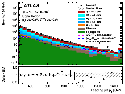
\includegraphics[width=\linewidth]{sr_jet1_pt}
    \caption{Leading jet $\pt$ distribution.}
    \label{fig:sr_jet1_pt}
  \end{subfigure}
  \caption{Distribution of the $\met$ and the leading jet $\pt$ for IM1 signal
    region compared with the background estimates from the background only fit
    in the control regions. The distributions of different signal models are
    superimposed for comparison. The contribution from the multi-jet and NCB
    background is negligible and not reported in the plot. In the ratio window
    the error bars include experimental and systematic uncertainties.}
  \label{fig:sr_plots}
\end{figure}
%%% Local Variables:
%%% mode: latex
%%% TeX-master: "../search_for_DM_LED_with_ATLAS"
%%% End:
